\documentclass[a4paper,11pt]{article}

\usepackage[left=2.5cm,right=2.5cm,top=3cm,bottom=3cm,pdftex]{geometry}
\usepackage{amssymb, amsmath, url, natbib, float, subcaption, listings,mathtools}
\usepackage[utf8]{inputenc}
\usepackage[T1]{fontenc}
\usepackage[pdftex]{graphicx}

\DeclareGraphicsExtensions{.png, .pdf, .jpg}
\usepackage[pdftex, colorlinks, linkcolor=blue, urlcolor=blue, citecolor=blue, pagecolor=blue, breaklinks=true]{hyperref}

\begin{document}

\pagestyle{empty}
\title{Comparison}
\begin{center}
\Large\textbf{CRAN packages comparison} \\[11pt]
\normalsize
\end{center}

\section{DiffusionRgqd}
Uses the cumulant truncation procedure developed by Varughese (2013), whereby the transition density can be approximated over arbitrarily large transition horizons for a suitably general class of non-linear diffusion models.

Generalized quadratic diffusions (GQD) are the specific class of SDEs with quadratic drift and diffusion terms:

\begin{align*}
d X_t & = \mu(X_t, t)dt + \sigma(X_t, t)dW_t, \: \text{where} \\
\mu(X_t, t) & = G_0(t) + G_1(t) X_t + G_2(t) X_t^2, \: \text{and} \\
\sigma (X_t, t) & = Q_0(t) + Q_1(t) X_t + Q_2(t) X_t^2
\end{align*}

For purposes of inference the drift and diffusion terms - and consequently the transitional density - are assumed to be dependent on a vector of parameters, $\theta$. For example, an Ornstein-Uhlenbeck model with SDE:

\begin{equation}
d X_t = \theta_1 (\theta_2 - X_t) + \sqrt{\theta_3^2} dW_t
\end{equation}

\begin{knitrout}
\definecolor{shadecolor}{rgb}{0.969, 0.969, 0.969}\color{fgcolor}\begin{kframe}
\begin{alltt}
\hlstd{G0}\hlkwb{=}\hlkwa{function}\hlstd{(}\hlkwc{t}\hlstd{)\{theta[}\hlnum{1}\hlstd{]}\hlopt{*}\hlstd{theta[}\hlnum{2}\hlstd{]\}}
\hlstd{G1}\hlkwb{=}\hlkwa{function}\hlstd{(}\hlkwc{t}\hlstd{)\{}\hlopt{-}\hlstd{theta[}\hlnum{1}\hlstd{]\}}
\hlstd{Q0}\hlkwb{=}\hlkwa{function}\hlstd{(}\hlkwc{t}\hlstd{)\{theta[}\hlnum{3}\hlstd{]}\hlopt{*}\hlstd{theta[}\hlnum{3}\hlstd{]\}}
\end{alltt}
\end{kframe}
\end{knitrout}

\subsection{Constant drift, diffusion SDE}
For a constant drift, diffusion SDE, with given initial condition $X_s$:
\begin{equation}
dX_t = \mu dt + \sigma dW_t
\end{equation}
The distribution at time $t$ of the process $X_t$ is $\mathcal{N}(X_t, X_s + \mu(t-s), \sigma^2(t-s))$

\begin{knitrout}
\definecolor{shadecolor}{rgb}{0.969, 0.969, 0.969}\color{fgcolor}\begin{kframe}
\begin{alltt}
\hlkwd{library}\hlstd{(}\hlstr{'DiffusionRgqd'}\hlstd{)}
\end{alltt}


{\ttfamily\noindent\bfseries\color{errorcolor}{\#\# Error in library("{}DiffusionRgqd"{}): there is no package called 'DiffusionRgqd'}}\begin{alltt}
\hlcom{# Remove any existing coefficients}
\hlkwd{GQD.remove}\hlstd{()}
\end{alltt}


{\ttfamily\noindent\bfseries\color{errorcolor}{\#\# Error in eval(expr, envir, enclos): could not find function "{}GQD.remove"{}}}\begin{alltt}
\hlstd{Xs} \hlkwb{<-} \hlnum{0}                 \hlcom{# Initial state}
\hlstd{Xt} \hlkwb{<-} \hlkwd{seq}\hlstd{(}\hlopt{-}\hlnum{3}\hlopt{/}\hlnum{2}\hlstd{,}\hlnum{3}\hlopt{/}\hlnum{2}\hlstd{,}\hlnum{1}\hlopt{/}\hlnum{50}\hlstd{)}\hlcom{# Possible future states}
\hlstd{s}  \hlkwb{<-} \hlnum{0}                 \hlcom{# Starting time}
\hlstd{t}  \hlkwb{<-} \hlnum{1}                 \hlcom{# Final time}
\hlstd{mu}    \hlkwb{<-} \hlnum{0.5}            \hlcom{# Drift parameter}
\hlstd{sigma} \hlkwb{<-} \hlnum{0.25}           \hlcom{# Diffusion coefficient}

\hlcom{# Define the model coefficients}
\hlstd{G0} \hlkwb{<-} \hlkwa{function}\hlstd{(}\hlkwc{t}\hlstd{)\{mu\}}
\hlstd{Q0} \hlkwb{<-} \hlkwa{function}\hlstd{(}\hlkwc{t}\hlstd{)\{sigma}\hlopt{^}\hlnum{2}\hlstd{\}}

\hlcom{# Calculate the transitional density}
\hlstd{BM} \hlkwb{<-} \hlkwd{GQD.density}\hlstd{(Xs,Xt,s,t)}
\end{alltt}


{\ttfamily\noindent\bfseries\color{errorcolor}{\#\# Error in eval(expr, envir, enclos): could not find function "{}GQD.density"{}}}\begin{alltt}
\hlcom{# Plot the transitional density}
\hlkwd{plot}\hlstd{(}\hlkwd{dnorm}\hlstd{(Xt, Xs}\hlopt{+}\hlstd{mu}\hlopt{*}\hlstd{(t}\hlopt{-}\hlstd{s), sigma}\hlopt{*}\hlkwd{sqrt}\hlstd{(t}\hlopt{-}\hlstd{s))}\hlopt{~}\hlstd{Xt,} \hlkwc{main} \hlstd{=} \hlstr{'Transition density'}\hlstd{,} \hlkwc{type} \hlstd{=} \hlstr{'l'}\hlstd{)}
\end{alltt}
\end{kframe}
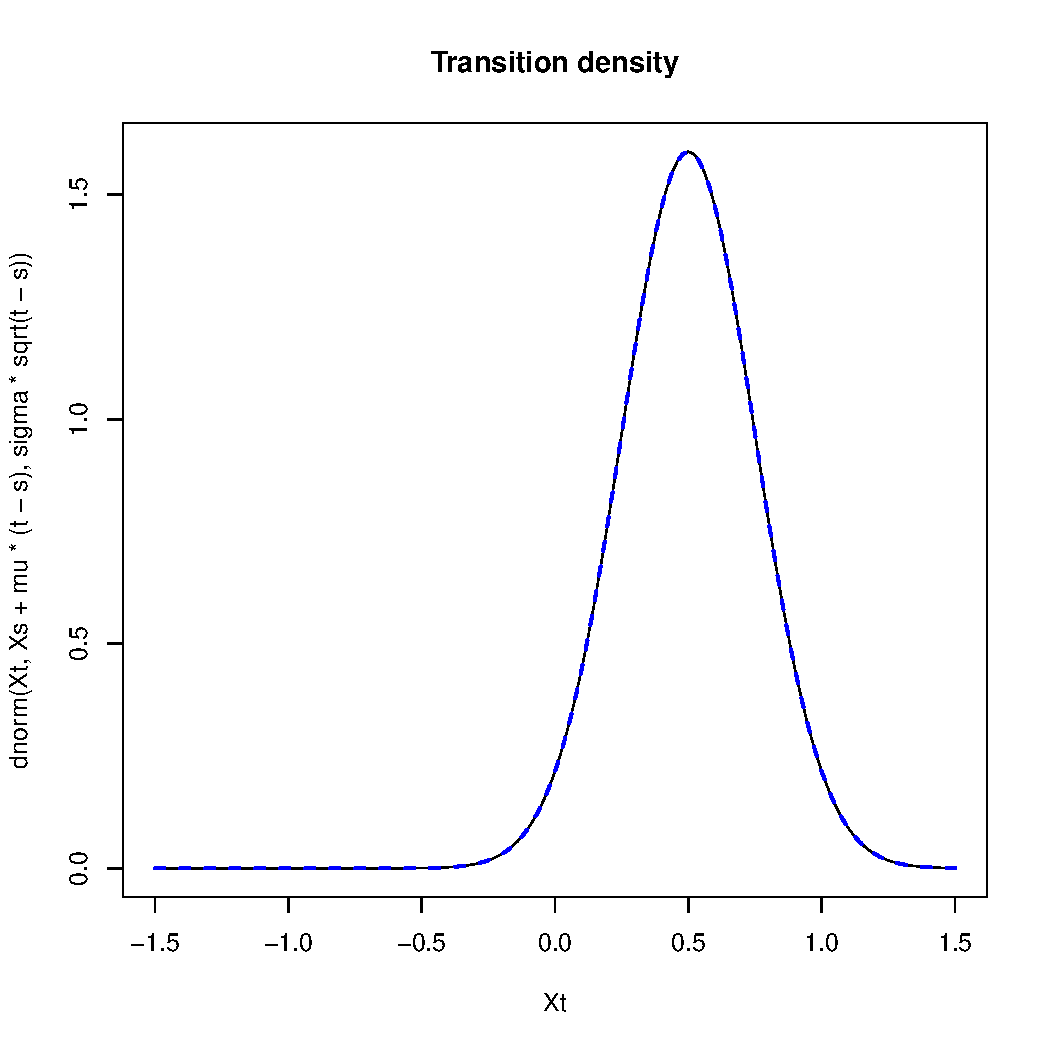
\includegraphics[width=4in,height=4in]{figure/GQD-brownian-1} 
\begin{kframe}\begin{alltt}
\hlkwd{lines}\hlstd{(BM}\hlopt{$}\hlstd{density[,}\hlnum{100}\hlstd{]}\hlopt{~}\hlstd{BM}\hlopt{$}\hlstd{Xt,} \hlkwc{col} \hlstd{=} \hlstr{'blue'}\hlstd{,} \hlkwc{lty} \hlstd{=} \hlstr{'dashed'}\hlstd{,} \hlkwc{lwd} \hlstd{=} \hlnum{2}\hlstd{)}
\end{alltt}


{\ttfamily\noindent\bfseries\color{errorcolor}{\#\# Error in eval(expr, envir, enclos): object 'BM' not found}}\end{kframe}
\end{knitrout}

\subsection{CIR process}
Another example using the CIR process SDE:
\begin{equation}
dX_t = \theta_1 (\theta_2 - X_t)dt + \theta_3 \sqrt{X_t} dW_t
\end{equation}

\begin{knitrout}
\definecolor{shadecolor}{rgb}{0.969, 0.969, 0.969}\color{fgcolor}\begin{kframe}
\begin{alltt}
\hlkwd{GQD.remove}\hlstd{()}
\end{alltt}


{\ttfamily\noindent\bfseries\color{errorcolor}{\#\# Error in eval(expr, envir, enclos): could not find function "{}GQD.remove"{}}}\begin{alltt}
\hlstd{a} \hlkwb{=} \hlnum{0.5}\hlstd{; b} \hlkwb{=} \hlnum{5}\hlstd{; sigma} \hlkwb{=} \hlnum{0.35}\hlstd{;} \hlcom{# Parameter values}

\hlstd{G0} \hlkwb{<-} \hlkwa{function}\hlstd{(}\hlkwc{t}\hlstd{)\{a}\hlopt{*}\hlstd{b\}}
\hlstd{G1} \hlkwb{<-} \hlkwa{function}\hlstd{(}\hlkwc{t}\hlstd{)\{}\hlopt{-}\hlstd{a\}}
\hlstd{Q1} \hlkwb{<-} \hlkwa{function}\hlstd{(}\hlkwc{t}\hlstd{)\{sigma}\hlopt{^}\hlnum{2}\hlstd{\}}

\hlstd{states}     \hlkwb{<-}  \hlkwd{seq}\hlstd{(}\hlnum{1}\hlstd{,} \hlnum{9}\hlstd{,} \hlnum{1}\hlopt{/}\hlnum{10}\hlstd{)}\hlcom{# State values}
\hlstd{initial}    \hlkwb{<-}  \hlnum{6}              \hlcom{# Starting value of the process}
\hlstd{Tmax}       \hlkwb{<-}  \hlnum{5}              \hlcom{# Time horizon}
\hlstd{Tstart}     \hlkwb{<-}  \hlnum{1}              \hlcom{# Time starts at 1}
\hlstd{increment}  \hlkwb{<-}  \hlnum{1}\hlopt{/}\hlnum{100}          \hlcom{# Incremental time steps}

\hlcom{# Generate the transitional density}
\hlstd{M} \hlkwb{<-} \hlkwd{GQD.density}\hlstd{(}\hlkwc{Xs} \hlstd{= initial,} \hlkwc{Xt} \hlstd{= states,} \hlkwc{s} \hlstd{= Tstart,} \hlkwc{t} \hlstd{= Tmax,} \hlkwc{delt} \hlstd{= increment)}
\end{alltt}


{\ttfamily\noindent\bfseries\color{errorcolor}{\#\# Error in eval(expr, envir, enclos): could not find function "{}GQD.density"{}}}\begin{alltt}
\hlkwd{persp}\hlstd{(}\hlkwc{x} \hlstd{= M}\hlopt{$}\hlstd{Xt,} \hlkwc{y} \hlstd{= M}\hlopt{$}\hlstd{time,} \hlkwc{z} \hlstd{= M}\hlopt{$}\hlstd{density,} \hlkwc{col} \hlstd{=} \hlstr{'white'}\hlstd{,} \hlkwc{xlab} \hlstd{=} \hlstr{'State (X_t)'}\hlstd{,}\hlkwc{ylab}
 \hlstd{=} \hlstr{'Time (t)'}\hlstd{,} \hlkwc{zlab} \hlstd{=} \hlstr{'Density f(X_t|X_s)'}\hlstd{,} \hlkwc{border} \hlstd{=} \hlnum{NA}\hlstd{,} \hlkwc{shade} \hlstd{=} \hlnum{0.5}\hlstd{,} \hlkwc{theta} \hlstd{=} \hlnum{145}\hlstd{)}
\end{alltt}


{\ttfamily\noindent\bfseries\color{errorcolor}{\#\# Error in persp(x = M\$Xt, y = M\$time, z = M\$density, col = "{}white"{}, xlab = "{}State (X\_t)"{}, : object 'M' not found}}\end{kframe}
\end{knitrout}

























